% ------------------------------------------------------------------------------
% TYPO3 CMS 7.0 - What's New - Chapter "Introduction" (German Version)
%
% @author	Patrick Lobacher <patrick@lobacher.de>
% @license	Creative Commons BY-NC-SA 3.0
% @link		http://typo3.org/download/release-notes/whats-new/
% @language	German
% ------------------------------------------------------------------------------
% LTXE-CHAPTER-UID:		947f71fe-f93742b1-4879d61a-4a9bbcd6
% LTXE-CHAPTER-NAME:	Introduction
% ------------------------------------------------------------------------------

\section{Einführung}
\begin{frame}[fragile]
	\frametitle{Einführung}

	\begin{center}\huge{Einführung}\end{center}
	\begin{center}\huge{\color{typo3darkgrey}\textbf{(Die Fakten)}}\end{center}

\end{frame}

% ------------------------------------------------------------------------------
% LTXE-SLIDE-START
% LTXE-SLIDE-UID:		722604a4-1fd701f2-1adf8e9a-60d35921
% LTXE-SLIDE-ORIGIN:	xxxxxxxx-xxxxxxxx-xxxxxxxx-xxxxxxxx
% LTXE-SLIDE-TITLE:		TYPO3 CMS 7.0 - Die Fakten
% ------------------------------------------------------------------------------

\begin{frame}[fragile]
	\frametitle{Einführung}
	\framesubtitle{TYPO3 CMS 7.0: Die Fakten}

	\begin{itemize}
		\item Veröffentlichungsdatum: 2. Dezember 2014
		\item Releasetyp: "Sprint Release"
		\item Vision: Embrace, Innovate, Deliver
		\item Hauptfokus: Generalüberholung des Backends
	\end{itemize}

	\begin{figure}
		
\includegraphics[width=0.95\linewidth]{typo3-seven-zero-banner.png}
	\end{figure}

\end{frame}

% ------------------------------------------------------------------------------
% LTXE-SLIDE-START
% LTXE-SLIDE-UID:		4d5ad4e7-09ffb1a1-e4649924-c52bd77a
% LTXE-SLIDE-ORIGIN:	xxxxxxxx-xxxxxxxx-xxxxxxxx-xxxxxxxx
% LTXE-SLIDE-TITLE:		Systemvoraussetzungen
% ------------------------------------------------------------------------------

\begin{frame}[fragile]
	\frametitle{Einführung}
	\framesubtitle{Systemvoraussetzungen}

	\begin{itemize}
		\item PHP*:\tabto{3cm}v5.5.0 - v5.6.x
		\item MySQL:\tabto{3cm}v5.5.x - v5.6.x (no strict mode)
		\item Festplattenplatz:\tabto{3cm}mindestens 200 MB
		\item PHP Einstellungen:

			\begin{itemize}
				\item memory\_limit >= 128M
				\item max\_execution\_time >= 240s
				\item PHP Kompilierungsoption \texttt{--disable-ipv6} darf \underline{nicht} aktiviert sein
			\end{itemize}

		\item Backend benötigt IE >= 9 oder jeden anderen modernen Browser

	\end{itemize}

	\vspace{1cm}
	*) weitere Details: \href{http://typo3.org/news/article/php-minimum-requirements-for-typo3-cms-7/}{PHP Minimum Requirements for TYPO3 CMS 7}

\end{frame}

% ------------------------------------------------------------------------------
% LTXE-SLIDE-START
% LTXE-SLIDE-UID:		502df190-810d99c2-c261f8e8-23ba520c
% LTXE-SLIDE-ORIGIN:	xxxxxxxx-xxxxxxxx-xxxxxxxx-xxxxxxxx
% LTXE-SLIDE-TITLE:		Neuer Release-Zyklus
% ------------------------------------------------------------------------------

\begin{frame}[fragile]
	\frametitle{Einführung}
	\framesubtitle{Neuer Release-Zyklus}

	\begin{figure}
		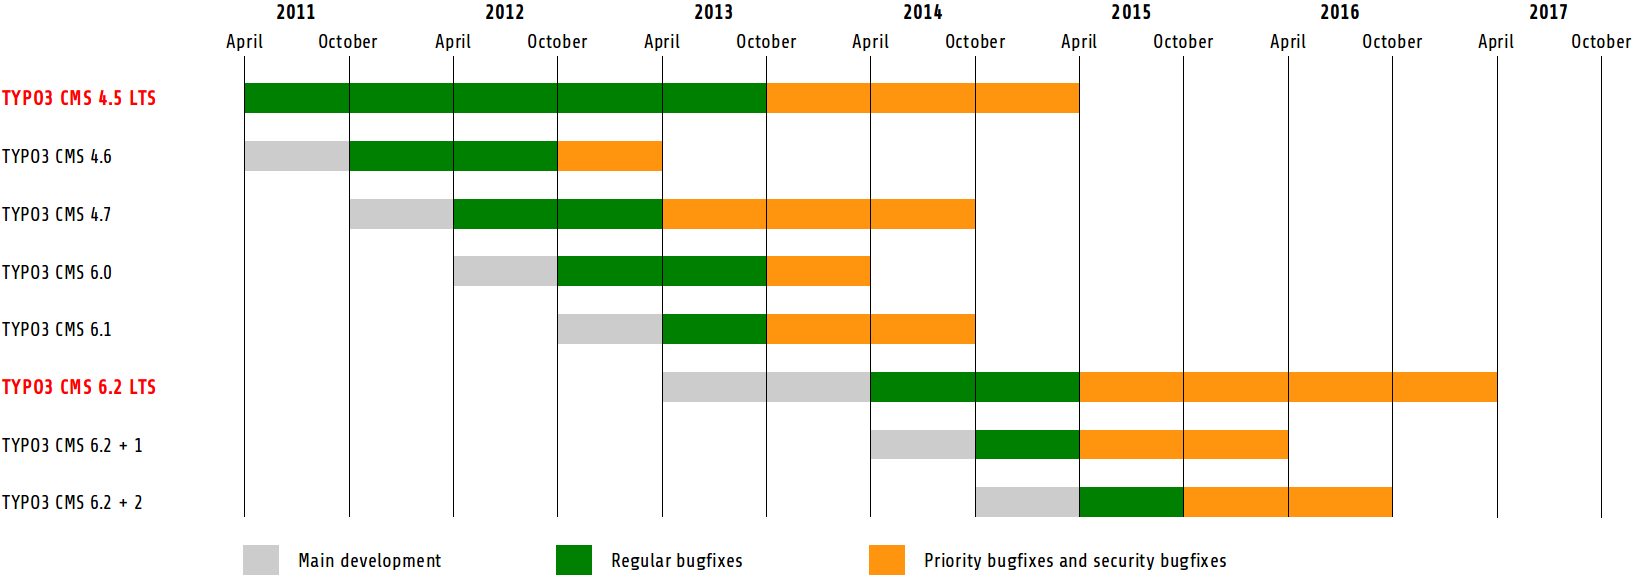
\includegraphics[width=0.90\linewidth]{Introduction/ReleaseAgenda.png}
	\end{figure}

\end{frame}

% ------------------------------------------------------------------------------
% LTXE-SLIDE-START
% LTXE-SLIDE-UID:		e7758148-7a5e4668-be46a5e3-fcfbddaf
% LTXE-SLIDE-ORIGIN:	xxxxxxxx-xxxxxxxx-xxxxxxxx-xxxxxxxx
% LTXE-SLIDE-TITLE:		Roadmap
% ------------------------------------------------------------------------------
% https://typo3.org/typo3-cms/roadmap/

\begin{frame}[fragile]
	\frametitle{Einführung}
	\framesubtitle{TYPO3 CMS Roadmap}

	Voraussichtliche Veröffentlichungen und deren Hauptfokus:

	\begin{itemize}
		\item
			\begingroup
				\color{typo3orange}
					v7.0 \textrightarrow\tabto{1.3cm}02/Dez/2014\tabto{3.4cm}Backend Overhaul Vol 1
			\endgroup

		\item v7.1 \textrightarrow\tabto{1.3cm}17/Feb/2015\tabto{3.4cm}Core Cleanup \& Streamlining
		\item v7.2 \textrightarrow\tabto{1.3cm}10/Mär/2015\tabto{3.4cm}Frontend
		\item v7.3 \textrightarrow\tabto{1.3cm}21/Apr/2015\tabto{3.4cm}Composer Ecosystem
		\item v7.4 \textrightarrow\tabto{1.3cm}09/Jun/2015\tabto{3.4cm}Backend Overhaul Vol 2
		\item v7.5 \textrightarrow\tabto{1.3cm}28/Jul/2015\tabto{3.4cm}\textit{(noch unbestimmt)}
		\item v7.6 \textrightarrow\tabto{1.3cm}13/Okt/2015\tabto{3.4cm}pre-LTS inferno
		\item v7.7 \textrightarrow\tabto{1.3cm}xx/xxx/2015\tabto{3.4cm}\textbf{TYPO3 CMS 7 LTS} (Long Term Release)
	\end{itemize}

	\smaller
		\url{https://typo3.org/typo3-cms/roadmap/}\newline
		\url{http://typo3.org/news/article/embrace-and-innovate-typo3-cms-7/}
	\normalsize

\end{frame}

% ------------------------------------------------------------------------------
% LTXE-SLIDE-START
% LTXE-SLIDE-UID:		847ffbc6-c2c8bfd2-6da2f8b4-f3e32a7d
% LTXE-SLIDE-ORIGIN:	xxxxxxxx-xxxxxxxx-xxxxxxxx-xxxxxxxx
% LTXE-SLIDE-TITLE:		Installation
% LTXE-SLIDE-REFERENCE:	https://forge.typo3.org/issues/62578
% ------------------------------------------------------------------------------

\begin{frame}[fragile]
	\frametitle{Einführung}
	\framesubtitle{Installation}

	\begin{itemize}
		\item Empfohlene Installationsschritte unter Linux/Mac OS X\newline
			(DocumentRoot ist beispielsweise \texttt{/var/www/site/htdocs}):
		\begin{lstlisting}
			$ cd /var/www/site
			$ wget --content-disposition get.typo3.org/7.0
			$ tar xzf typo3_src-7.0.0.tar.gz
			$ cd htdocs
			$ ln -s ../typo3_src-7.0.0 typo3_src
			$ ln -s typo3_src/index.php
			$ ln -s typo3_src/typo3
			$ touch FIRST_INSTALL
		\end{lstlisting}

		\item Symbolische Links unter Microsoft Windows:

			\begin{itemize}
				\item unter Windows XP/2000 kann \texttt{junction} benutzt werden
				\item unter Windows Vista und Windows 7 kann \texttt{mlink} benutzt werden
			\end{itemize}

	\end{itemize}
\end{frame}

% ------------------------------------------------------------------------------
% LTXE-SLIDE-START
% LTXE-SLIDE-UID:		c1084a3b-355d016d-83d31a7e-ef5089a3
% LTXE-SLIDE-ORIGIN:	xxxxxxxx-xxxxxxxx-xxxxxxxx-xxxxxxxx
% LTXE-SLIDE-TITLE:		Upgrade zu TYPO3 CMS 7
% LTXE-SLIDE-REFERENCE:	https://forge.typo3.org/issues/62578
% ------------------------------------------------------------------------------

\begin{frame}[fragile]
	\frametitle{Einführung}
	\framesubtitle{Upgrade zu TYPO3 CMS 7}

	\begin{itemize}
		\item Upgrades nur von TYPO3 CMS 6.2 LTS möglich
		\item TYPO3 CMS < 6.2 sollte man erst auf TYPO3 CMS 6.2 LTS aktualisieren
	\end{itemize}

	\begin{itemize}

		\item Upgrade-Anleitung:\newline
			\smaller\url{http://wiki.typo3.org/Upgrade#Upgrading_to_7.0}\normalsize
		\item Offizielles TYPO3 Guide "TYPO3 Installation and Upgrading":
			\smaller\url{http://docs.typo3.org/typo3cms/InstallationGuide}\normalsize
		\item Generelles Vorgehen:
			\begin{itemize}
				\item Prüfen, ob Mindestvoraussetzungen erfüllt sind \small(PHP, MySQL, etc.)
				\item Das \textbf{deprecation\_*.log} der TYPO3 Instanz durchsehen
				\item Sämtliche Extensions auf den aktuellsten Stand bringen
				\item Neuen TYPO3 Quellcode entpacken und im Install Tool den Upgrade Wizard ausführen
				\item Startup Modul von Backend Benutzern überprüfen (optional)
			\end{itemize}
	\end{itemize}

\end{frame}

% ------------------------------------------------------------------------------
